\documentclass[oneside,onecolumn,12pt]{report}
\bibliographystyle{IEEEtran}

% Include first: order-sensitive packages
\usepackage[dvipdfmx]{graphicx,xcolor,hyperref}
\usepackage{ascmac}

% English font (Use Latin Modern instead of Computer Modern)
\usepackage[T1]{fontenc}
\usepackage{lmodern}

\usepackage{algorithm}
\usepackage{algpseudocode}
\usepackage{amsfonts}
\usepackage{amsmath}
\usepackage{amssymb}
\usepackage{bm}
\usepackage{caption}
\usepackage{cite}
\usepackage{comment}
\usepackage{fancybox}
\usepackage{float}
\usepackage{geometry}
\usepackage{latexsym}
\usepackage{layout}
\usepackage{multirow}
\usepackage{nidanfloat}
\usepackage{paralist}
\usepackage{pifont}
\usepackage{pxjahyper}
\usepackage{tabularx}
\usepackage{tocloft}
\usepackage{url}

% For thesis written in English
\usepackage{thesisen}


%%%%%%%%%%%%%%%%%%%%%%%%%%%%%%%%%%%%%%%%%%%%%%%%%%%%%%%%%%%%%%%%%%%%%%%
%%
%% Personal Settings
%%
%%%%%%%%%%%%%%%%%%%%%%%%%%%%%%%%%%%%%%%%%%%%%%%%%%%%%%%%%%%%%%%%%%%%%%%

% See: http://hurou927.hatenablog.com/entry/2015/06/25/142126
\newcolumntype{C}{>{\centering\arraybackslash}X}
\newcolumntype{L}{>{\raggedright\arraybackslash}X}
\newcolumntype{R}{>{\raggedleft\arraybackslash}X}

% Python-like pseudocode
\algrenewcommand\algorithmicrequire{\textbf{Input:}}
\algrenewcommand\algorithmicensure{\textbf{Output:}}
\newcommand{\abs}[1]{\lvert #1 \rvert}
\newcommand{\Break}{\textbf{break}}
\renewcommand{\Return}{\textbf{return }}
\makeatletter\renewcommand*{\ALG@name}{Algorithm}\makeatother
\algtext*{EndFunction}
\algtext*{EndWhile}
\algtext*{EndFor}
\algtext*{EndIf}


%%%%%%%%%%%%%%%%%%%%%%%%%%%%%%%%%%%%%%%%%%%%%%%%%%%%%%%%%%%%%%%%%%%%%%%
%%
%% Contents of This Thesis
%%
%%%%%%%%%%%%%%%%%%%%%%%%%%%%%%%%%%%%%%%%%%%%%%%%%%%%%%%%%%%%%%%%%%%%%%%

\begin{document}

% \layout  % For debugging page layout

\MyTitleA{Answer to the Ultimate Question}
\MyTitleB{of}
\MyTitleC{Life, the Universe, and Everything}
\MyName{Taro SHURON}
\MySupervisor{Katsunori YAMAOKA}
\MyDegreeType{M}
\MonthYear{January 2020}

% Left binding support
%   Y: Margin left=38mm, right=22mm (for bookbinding)
%   N: Margin left=30mm, right=30mm (for PDF export)
\LeftBinding{N}

\maketitle
\makepagestyle  % Set style for thesis

\pagenumbering{roman}
\setcounter{page}{1}

\addcontentsline{toc}{chapter}{Abstract}
% !TEX root = ../main.tex
\chapter*{Abstract}
The main contribution of this thesis is summarized as follows: achievement of my happy graduation.

\clearpage

\addcontentsline{toc}{chapter}{Acknowledgement}
% !TEX root = ../main.tex
\chapter*{Acknowledgement}

I would like to express the most in-depth appreciation to my supervisor Prof. Katsunori Yamaoka and Prof. Yoshiaki Kitaguchi.
Special thanks to Mrs. Matsuzaki and all the members of Yamaoka-Kitaguchi Laboratory for all the fun, help, and support.
Finally, I am indebted to my family members for their full and unconditional support for all these years.

\clearpage

\setcounter{tocdepth}{2}

\addcontentsline{toc}{chapter}{Table of Contents}
\tableofcontents
\clearpage

\addcontentsline{toc}{chapter}{List of Figures}
\listoffigures
\clearpage

\addcontentsline{toc}{chapter}{List of Tables}
\listoftables
\clearpage

\pagenumbering{arabic}
\setcounter{page}{1}

% !TEX root = ../main.tex
\chapter{Introduction} \label{sec:introduction}

\begin{figure}[h]
 \vspace{5mm}
 \centering
 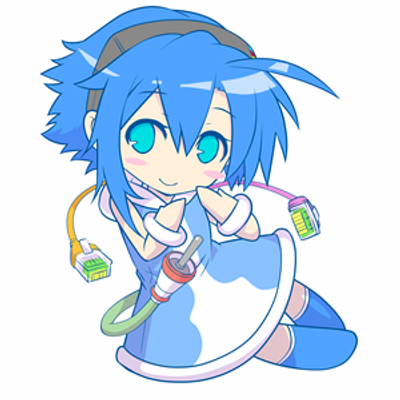
\includegraphics[width=100mm]{figures/tech-chan.png}
 \caption{Kawaii.}
 \label{fig:tech-chan}
 \vspace{5mm}
\end{figure}

\clearpage

% !TEX root = ../main.tex
\chapter{Related Work} \label{sec:relatedwork}
Yamaoka et al. proposed a novel routing algorithm based on game theory \cite{yamaoka}.

\clearpage

% !TEX root = ../main.tex
\chapter{System Model and Problem Statement} \label{sec:model}

\clearpage

% !TEX root = ../main.tex
\chapter{Proposed Method} \label{sec:algorithm}

\clearpage

% !TEX root = ../main.tex
\chapter{Performance Evaluation} \label{sec:analysis}

\clearpage

% !TEX root = ../main.tex
\chapter{Conclusion and Future Work} \label{sec:conclusion}

\clearpage

\setstretch{1.2}
\addcontentsline{toc}{chapter}{Bibliography}
\bibliography{library.bib}
\clearpage

\pagenumbering{roman}
\setcounter{page}{8}

\addcontentsline{toc}{chapter}{Colophon}
% !TEX root = ../main.tex
\chapter*{Colophon}

\begin{table}[H]
  \setstretch{1.0}
  \large
  \begin{tabularx}{155mm}{ll}
    {\normalsize 英文題目} & \begin{tabular}{l} The Answer to the Ultimate Question of Life, the Universe,\\and Everything \end{tabular} \\[4ex]
    {\normalsize 和文題目} & \begin{tabular}{l} 生命・宇宙・そして万物についての究極の疑問の答え \end{tabular} \\[4ex]
    {\normalsize 氏名} &     \begin{tabular}{l} 修論 太郎 \end{tabular} \\[2ex]
    {\normalsize 学籍番号} & \begin{tabular}{l} 18M12345 \end{tabular} \\[2ex]
    {\normalsize 所属} &     \begin{tabular}{l} 工学院情報通信系 情報通信コース\\山岡研究室 \end{tabular} \\[4ex]
    {\normalsize 指導教員} & \begin{tabular}{l} 山岡 克式 教授 \end{tabular} \\[2ex]
    {\normalsize 入学年月} & \begin{tabular}{l} 2018年4月\end{tabular} \\[2ex]
    {\normalsize 修了年月} & \begin{tabular}{l} 2020年3月(2020年1月提出) \end{tabular} \\[2ex]
  \end{tabularx}
\end{table}

\clearpage

\end{document}
